\documentclass[10pt,a4paper]{amsart}
\usepackage{amsmath,amssymb,amsthm,graphicx}
\usepackage{hyperref}
\usepackage{tikz}
\usepackage[all]{xy}

\usetikzlibrary{arrows.meta}

\usetikzlibrary{shapes.misc}
\usetikzlibrary{decorations.pathmorphing}

\usepackage{euscript}


\DeclareMathOperator{\Aut}{Aut}
\DeclareMathOperator{\Bir}{Bir}
\DeclareMathOperator{\Auteq}{Auteq}
\DeclareMathOperator{\Ext}{Ext}
\DeclareMathOperator{\Quad}{Quad}

\def\CH{\mathrm{CH}}
\newcommand {\Coh} {\operatorname{Coh}}
\newcommand {\ccoh} {\operatorname{coh}}
\def\etaX{\eta}
\def\bc{\mathrm{bc}}
\def\ls{\mathrm{ls}}


\newcommand{\Sch}{\mathrm{Sch}}
\newcommand{\Sets}{\mathrm{Sets}}
\newcommand{\Spec}{\mathrm{Spec}}
\newcommand{\Sym}{\mathrm{Sym}}
\newcommand{\Cob}{\mathrm{Cob}}
\newcommand{\Sph}{\mathrm{Sph}}
\newcommand{\Ham}{\mathrm{Ham}}
\newcommand{\FS}{\mathrm{FS}}
\newcommand{\std}{\mathrm{std}}
\newcommand{\Bl}{\mathrm{Bl}}
\newcommand{\Adm}{\mathrm{Adm}}

\newcommand{\st}{\mathrm{st}}
\newcommand{\ct}{\mathrm{ct}}
\newcommand{\Tw}{\mathrm{Tw}}
%\newcommand{\tw}{\mathrm{tw}}
\def\BC{\mathrm{BC}}
\def\LS{\mathrm{LS}}
\def\bimod{\text{-mod-}}
\def\lmod{\text{-mod}}
\def\rmod{\text{mod-}}
\def\yon{\mathcal{Y}}
\def\specm{\mathsf{Spec}_\fm}
\def\fm{\mathfrak{m}}
\def\d{\mathbf{d}}

\newcommand{\scrM}{\EuScript{M}}
\def\scrA{\EuScript{A}}
\def\scrJ{\EuScript{J}}

\def\scrK{\EuScript{K}}

\def\scrP{\EuScript{P}}
\def\scrQ{\EuScript{Q}}
\def\scrR{\EuScript{R}}
\def\scrN{\EuScript{N}}
\def\cL{\EuScript{L}}
\def\cO{\EuScript{O}}
\def\cT{\EuScript{T}}
\newcommand{\scrF}{\EuScript{F}}
\newcommand{\scrC}{\EuScript{C}}
\newcommand{\scrE}{\EuScript{E}}
\def\scrW{\EuScript{W}}
\def\scrHom{\mathcal{H}om}
\def\scrV{\EuScript{V}}

\DeclareMathOperator{\Diff}{Diff}

%\DeclareMathOperator{\Bir}{Bir}
\DeclareMathOperator{\Symp}{Symp}
\DeclareMathOperator{\Stab}{Stab}
\def\P{\mathcal{P}}
\newcommand{\NS}{\operatorname{NS}}
\newcommand{\per}{\operatorname{per}}
\def\bK{\mathbb{K}}
\def\bP{\mathbb{P}}
\def\bA{\mathbb{A}}
\def\bB{\mathbb{B}}
\def\bG{\mathbb{G}}
\def\bZ{\mathbb{Z}}
\def\bQ{\mathbb{Q}}

\def\bC{\mathbb{C}}
\newcommand{\bS}{\mathbb{S}}
\def\Db{\mathop{\rm{D}^b}\nolimits}

\def\bT{\mathbb{T}}
\def\bR{\mathbb{R}}
\def\bL{\mathbb{L}}
\def\calR{\mathcal{R}}
\def\calS{\mathcal{S}}
\def\bN{\mathbb{N}}
\def\bV{\mathbb{V}}
\def\cU{\mathcal{U}}
\def\cC{\mathcal{C}}
\def\calL{\mathcal{L}}

\def\cZ{\mathcal{Z}}
\def\A{A}
\def\scrD{\EuScript{D}}
\def\scrL{\EuScript{L}}
\def\scrG{\EuScript{G}}
\def\scrS{\EuScript{S}}

\def\sph{V}
\DeclareMathOperator{\Pic}{Pic}

\newcommand{\id}{\mathrm{id}}

\newcommand{\KS}{\mathsf{KS}}
\def\pol{\Delta}
\def\val{\mathrm{val}}

\def\unob{\mathrm{unob}}

\newcommand{\rk}{\operatorname{rk}}

\newcommand{\power}[1]{\left[\!\left[ #1 \right]\!\right]}
\newcommand{\laurents}[1]{\left(\!\left( #1 \right)\!\right)}
\def\trop{\mathrm{trop}}

%\usepackage[T1]{fontenc}
\usepackage{mathabx,graphicx}
\def\Circlearrowleft{\ensuremath{%
 \rotatebox[origin=c]{180}{$\circlearrowleft$}}}
\def\Circlearrowright{\ensuremath{%
 \rotatebox[origin=c]{180}{$\circlearrowright$}}}


\newtheorem{thm}{Theorem}[section]
\newtheorem{lem}[thm]{Lemma}
\newtheorem{prop}[thm]{Proposition}
\newtheorem{cor}[thm]{Corollary}
\newtheorem{qn}[thm]{Question}
\newtheorem{conj}[thm]{Conjecture}
\newtheorem{assum}[thm]{Assumption}

\theoremstyle{definition}
\newtheorem{defn}[thm]{Definition}
\newtheorem{ex}[thm]{Example}
\newtheorem{rmk}[thm]{Remark}
\newtheorem*{rks}{Remarks}

%\newenvironment{pf}{ \begin{proof} }{ \end{proof} }

\newcommand\Hom{\operatorname{\mathsf{Hom}}}
\renewcommand\det{\operatorname{\mathsf{det}}}
\DeclareMathOperator{\rank}{\mathsf{rank}}
\DeclareMathOperator{\coh}{\mathsf{Coh}}
\DeclareMathOperator{\der}{\mathsf{D}}
\DeclareMathOperator{\dersplit}{\mathsf{D}^\pi}
\DeclareMathOperator{\VB}{\mathsf{vect}}
\DeclareMathOperator{\cx}{\mathsf{Ch}}
\DeclareMathOperator{\tw}{\mathsf{tw}}
\DeclareMathOperator{\twsplit}{\mathsf{tw}^\pi}
\DeclareMathOperator{\perf}{\mathsf{Perf}}
\DeclareMathOperator{\QC}{\mathsf{QC}}
\DeclareMathOperator{\spec}{\mathsf{Spec}}
\DeclareMathOperator{\proj}{\mathsf{Proj}}
\DeclareMathOperator{\ext}{\mathsf{Ext}}
\DeclareMathOperator{\HH}{\mathsf{HH}}
\DeclareMathOperator{\ch}{\mathsf{char}}
\DeclareMathOperator{\ob}{\mathsf{ob}}
\DeclareMathOperator{\modules}{\mathsf{mod}\text{-}}
\DeclareMathOperator{\Modules}{\mathsf{Mod}\text{-}}
\DeclareMathOperator{\auteq}{\mathsf{auteq}}
\DeclareMathOperator{\deriv}{\mathsf{Der}}
\DeclareMathOperator{\h}{\mathsf{H}}
\DeclareMathOperator{\RHom}{\mathsf{R\, Hom}}
\DeclareMathOperator{\RR}{\mathsf{R}}
\DeclareMathOperator{\spl}{\mathsf{spl}}
\DeclareMathOperator{\SheafEnd}{\underline{\sf{End}}}
\DeclareMathOperator{\SheafHom}{\underline{\sf{Hom}}}
\DeclareMathOperator{\SheafExt}{\underline{\sf{Ext}}}
\DeclareMathOperator{\perfdg}{\mathsf{perf}}
\DeclareMathOperator{\Res}{\mathsf{Res}}



\newcommand{\EuA}{\EuScript{A}}
\newcommand{\EuB}{\EuScript{B}}
\newcommand{\EuC}{\EuScript{C}}
\newcommand{\EuD}{\EuScript{D}}
\newcommand{\EuE}{\EuScript{E}}
\newcommand{\EuF}{\EuScript{F}}
\newcommand{\EuG}{\EuScript{G}}
\newcommand{\EuH}{\EuScript{H}}
\newcommand{\EuI}{\EuScript{I}}
\newcommand{\EuJ}{\EuScript{J}}
\newcommand{\EuK}{\EuScript{K}}
\newcommand{\EuL}{\EuScript{L}}
\newcommand{\EuM}{\EuScript{M}}
\newcommand{\EuN}{\EuScript{N}}
\newcommand{\EuO}{\EuScript{O}}
\newcommand{\EuP}{\EuScript{P}}
\newcommand{\EuQ}{\EuScript{Q}}
\newcommand{\EuR}{\EuScript{R}}
\newcommand{\EuS}{\EuScript{S}}
\newcommand{\EuT}{\EuScript{T}}
\newcommand{\EuU}{\EuScript{U}}
\newcommand{\EuV}{\EuScript{V}}
\newcommand{\EuW}{\EuScript{W}}
\newcommand{\EuX}{\EuScript{X}}
\newcommand{\EuY}{\EuScript{Y}}
\newcommand{\EuZ}{\EuScript{Z}}

\numberwithin{equation}{section}
\usepackage{cleveref}
\crefname{originalsection}{original section}{original sections}
\Crefname{originalsection}{Original section}{Original sections}
\makeatletter
\newlabel{sec:marked-bordered-surfaces}{{4}{source}{}{sourcepointer-1}{}}
\newlabel{sec:marked-bordered-surfaces@cref}{{[originalsection][0][]4}{[1][0][]source}{}{}{}}
\makeatother
\crefname{originalsection}{original section}{original sections}
\Crefname{originalsection}{Original section}{Original sections}
\makeatletter
\newlabel{sec:birational-proj-plane}{{7}{source}{}{sourcepointer-2}{}}
\newlabel{sec:birational-proj-plane@cref}{{[originalsection][0][]7}{[1][0][]source}{}{}{}}
\makeatother
\title{Splitting of symplectic braid-group monodromy for type A Milnor fibres in every complex dimension at least three}
\author{Ailsa Keating, Ivan Smith, Michael Wemyss}
\date{doi:10.3842/SIGMA.2026.080; CC BY 4.0}
\begin{document}
\maketitle
\noindent\textit{Allowed standard prerequisites (editorial).}\begin{itemize}
\item Autoequivalence groups and connected stability spaces of type A Calabi-Yau categories. Ikeda Theorems7.15,7.16; Qiu-Woolf Theorems B; BS Theorem9.9, all cited precisely in author proof
\item Cluster categories and exchange-graph quotient. Baur-Marsh, BRT, King-QiuYu-cluster Theorem8.6
\item Koszul duality and Rabinowitz/cluster equivalence for Dynkin plumbings. AbSm-plumbing, Kalck-Yang, BJK Corollary1.4 and Lekili-Ueda as explicitly cited
\end{itemize}\medskip
\ifdefined\hypertarget\hypertarget{sourcepointer-1}{}\fi
\noindent\textit{Source reference.} Original section 4: algebra-geometry/sources/sigma-2026-080/native/sigma26-080.tex, source lines 665--665. A footnote points to the later discussion for an analogue of the already explicitly cited AbSm-plumbing/Kalck-Yang Koszul duality fact; the Milnor case is established via those named references and the complete local splitting chain is included.\par\medskip
\ifdefined\hypertarget\hypertarget{sourcepointer-2}{}\fi
\noindent\textit{Source reference.} Original section 7: algebra-geometry/sources/sigma-2026-080/native/sigma26-080.tex, source lines 1307--1307. Forward pointer in introductory categorical scope only, unrelated to the type A splitting proof.\par\medskip
\section{Flavours of Fukaya category}\label{Sec:flavours}

Let $(X,\omega)$ be a connected symplectic manifold with $2c_1(X)=0$. We will fix a Maslov cover of the Lagrangian Grassmannian, meaning that there is a well-defined group $\Symp^{\rm gr}(X)$ of graded symplectomorphisms, and a subgroup $\bZ \leq \Symp^{\rm gr}(X)$ generated by the shift (i.e., the fibrewise deck transformation). Recall from \cite[Lemma~2.4]{Seidel:graded} the following.

\begin{lem}
There is an exact sequence
\[
1 \to \bZ \to \Symp^{\rm gr}(X) \to \Symp(X) \to H^1(X;\bR).
\]
The final map is not a homomorphism but its kernel is a subgroup.
\end{lem}

\begin{lem}\label{lem:forgetting-gradings-splits}
Suppose that $X$ is non-compact. The forgetful map $\Symp^{\rm gr}(X) \to \Symp(X)$ is split over the subgroup $\Symp_{\rm ct}(X)$.
\end{lem}

\begin{proof} Take the unique gradings for symplectomorphisms which act trivially on the fibres of the Maslov cover near infinity.
\end{proof}

Let $(X,\omega)$ be a Liouville manifold, with contact type boundary, and assume $2c_1(X)=0$. We will be interested in all of
\begin{enumerate}\itemsep=0pt
\item[(1)] the compact Fukaya category $\scrF(X)$, with objects compact graded exact spin Lagrangians;
\item[(2)] the wrapped Fukaya category $\scrW(X)$, with objects graded exact spin Lagrangians which are cones over Legendrian submanifolds near infinity;
\item[(3)] the Rabinowitz Fukaya category $\scrR(X) := \scrW(X) / \scrW(X)^{\rm prop}$, which is the Verdier quotient of the (Yoneda image of the) wrapped category by its subcategory of proper modules.
\end{enumerate}

All three categories are defined over $\bZ$, and $\scrF(X) \subset \scrW(X)$ is a full and faithful subcategory. We say that `Koszul duality' holds for the compact and wrapped categories if $\scrF(X) \subset \scrW(X)$ is a Koszul dualising subcategory in the sense of \cite[Definition~2.12]{GGV}. This often holds for Weinstein manifolds obtained from plumbings of simply connected pieces. Concretely, the wrapped category of a Weinstein manifold admits a finite set of generators $\{T_i \mid 1 \leq i \leq N\}$ and one seeks a finite set of compact branes $\{L_i \mid 1 \leq i \leq N\}$ such that the total endomorphism algebras $\scrQ = \bigoplus_{i,j} HF^*(L_i,L_j)$ and $\scrA = \bigoplus_{i,j} HW^*(T_i,T_j)$, which are augmented over the semisimple ring $\Bbbk = \bigoplus_{i=1}^N \bK_i$ generated by the units of the objects, are $A_{\infty}$-Koszul dual, meaning
\[
\scrQ \simeq \Ext_{\scrA}(\Bbbk,\Bbbk), \qquad \scrA \simeq \Ext_{\scrQ}(\Bbbk,\Bbbk).
\]
In this setting, there is an equivalence \cite[Corollary~1.4]{GGV}
\[
\scrR(X) \simeq \scrW(X) / \scrF(X).
\]
This is the formulation we will encounter in practise, but the general algebraic construction of~$\scrR(X)$ from~$\scrW(X)$ in particular shows that autoequivalences of the latter act on the former.
 (In Section~\ref{sec:birational-proj-plane}, it will be important to work over~$\bC$, to incorporate $\bC^*$-valued local systems on Lagrangians.)

 Any autoequivalence of $\scrW(X)$ arising from a symplectomorphism of $X$ will preserve the compact category $\scrF(X)$, and hence induce an equivalence of $\scrR(X)$. For background on $\scrF(X)$, see \cite{Seidel:FCPLT}, and for background on $\scrW(X)$, see~\cite{Abouzaid-Seidel:Viterbo}; for background on derived localisation in general, see~\cite{Drinfeld}, and in the context of $\scrR(X)$ specifically, see~\cite{GGV}.

The Grothendieck group $K(\scrF(X))$ is the free abelian group on isomorphism classes of objects, modulo relations coming from exact triangles.
For later use, we define the `numerical Grothendieck group'
\begin{equation}\label{eqn:Knum}
K_{\rm num}(\scrF(X))
\end{equation}
to be the quotient of $K(\scrF(X))$ by the subgroup which is the radical of the Euler pairing, i.e., that generated by compact exact Lagrangians $L \in \mathrm{Ob}\,\scrF(X)$ for which $\chi(HF^*(L,\bullet)) = 0$ for every $\bullet \in \scrW(X)$.

We will be interested in actions of symplectomorphism groups on Fukaya categories. Especially for actions on the wrapped category, one needs some control of maps at infinity to ensure that (perhaps after isotopy) they preserve the class of Lagrangians which are conical\footnote{Or more generally geometrically bounded for a dissipative almost complex structure in the sense of Groman~\cite{Groman}.} at infinity. We say a symplectomorphism $\phi$ of a Liouville manifold $(X,{\rm d}\theta)$ is \emph{exact} if $\phi^*\theta = \theta + {\rm d}f$ for some $f\colon X \to \bR$, and \emph{strongly exact} if one can take $f$ to have compact support. Both notions have obvious graded analogues. It is classical that strongly exact maps act on the wrapped category. Write $\Symp_{\rm ex}(X)$ for the group of exact symplectomorphisms.

\begin{lem}\label{lem:acts}
 Assume that the Liouville manifold $X$ has finite type, so can be written as the completion of a Liouville domain $\mathring{X}$. Then
 \begin{enumerate}\itemsep=0pt
 \item[$(1)$] There is a homomorphism \smash{$\pi_0\Symp_{\rm ct}(X) \to \pi_0\Symp_{\rm ex}\bigl(\mathring{X}\bigr)$};
 \item[$(2)$] The group \smash{$\pi_0\Symp\bigl(\mathring{X}\bigr)$} acts on both $\scrF(X)$ and $\scrW(X)$.
 \end{enumerate}
\end{lem}

\begin{proof}
 For the first statement, conjugation by a suitably large Liouville flow will bring the support into $\mathring{X}$. We claim we can then deform to obtain an exact representative of the map. Let $\omega = {\rm d} \lambda$ be the Liouville form on $X$, and suppose we are given $\psi \in \Symp_{\rm ct} (X)$. We have $\psi^\ast \lambda - \lambda = \theta$, where $\theta$ is a closed one-form with compact support. Let~$V$ be the vector field which is symplectically dual to $-\theta$. This has compact support, and so is integrable for all time; let $\sigma_t$ denote its flow. Then applying Cartan's formula, we get that $\psi \circ \sigma_1 $ is an exact symplectomorphism. (Note that the proof of \cite[Lemma~1.1]{BEE} specialises to this argument in this case.)

 This construction can be performed in families, which shows that the inclusion
 \[
 \Symp_{\rm ct,ex}(X) \hookrightarrow \Symp_{\rm ct}(X)
 \]
 is a homotopy equivalence, so induces an isomorphism on $\pi_0$. On the other hand, there is then a forgetful map
 \[
 \Symp_{\rm ct,ex}(X) \to \Symp_{\rm ex}(\mathring{X})
 \]
 which induces a homomorphism on $\pi_0$. Combining these two gives the first statement.

 The second statement is exactly \cite[Corollary~2.4]{Keating-Smith} (cf.~\cite{KS:corr}, which in particular involves deforming a map of the Liouville domain to be exact, using a version of the argument given in the previous paragraphs).
\end{proof}

\begin{lem}
In the setting of Lemma~{\rm \ref{lem:acts}}, assume moreover that $2c_1(\mathring{X})=0$.
Then there are compatible representations
\[
\xymatrix{
\pi_0\Symp^{\rm gr}_{\rm ct}(X) \ar[rr] \ar[d] && \Auteq(\scrF(X)) \\
\pi_0\Symp^{\rm gr}(\mathring{X}) \ar[rr] && \Auteq(\scrW(X)). \ar[u]
}
\]
\end{lem}
The top line is classical; the bottom line is \cite[Corollary~2.9]{Keating-Smith} (see also~\cite{KS:corr}).


Although the Rabinowitz category is not a priori determined by the contact boundary of $X$, one still has the following lemma.

\begin{lem}\label{lem:trivial on Rabinowitz}
The group $\pi_0\Symp^{\rm gr}_{\rm ct}(X)$ acts trivially on the Rabinowitz category.
\end{lem}

\begin{proof}
Let $L$, $K$ be Lagrangians which are cones over Legendrian submanifolds $L_{\infty}$ and $K_{\infty}$.
The morphism group ${RFC}^*(L,K)$ in $\scrR(X)$ between $L$ and $K$ is the chain-level mapping cone of a natural continuation map ${CW}_*(L,K) \to {CW}^*(L,K)$ coming from a monotone homotopy of Hamiltonians from `infinite negative wrapping to infinite positive wrapping'. This factors as a composition
\[
\xymatrix{
{CW}_*(L,K) \ar[r]_-a & {CF}^*(L,\phi_{-\varepsilon}K) \ar[r]_-c &
{CF}^*(L,\phi_{+\varepsilon}K) \ar[r]_-b & {CW}^*(L,K),
}
\]
where $a$, $b$ are projection respectively inclusion maps of summands into the relevant direct systems and $c$ is the natural continuation from small negative to small positive wrapping. Viewing ${RFC}^*(L,K) = \mathrm{Cone}(b\circ c \circ a)$,
there are exact triangles of mapping cones
\[
\mathrm{Cone}(c\circ a) \to {RFC}^*(L,K) \to \mathrm{Cone}(b)
\]
and
\[
\mathrm{Cone}(a) \to \mathrm{Cone}(c\circ a) \to \mathrm{Cone}(c).
\]
The continuation map $c$ induces the Poincar\'e duality isomorphism in Lagrangian Floer theory
\[
HF^*(L,\phi_{-\varepsilon}K) \to HF^*(L,\phi_{+\varepsilon}(K))
\]
(which recovers the isomorphism $H_*(L,\partial_{\infty}L) \to H^{n-*}(L)$ when $L=K$),
so has acyclic cone. On the other hand, $\mathrm{Cone}(b) \simeq {CW}(L,K)^+$ defines the Lagrangian Floer analogue of `positive symplectic cohomology' \cite{Ritter}; it can be computed by an action truncated version of the wrapped Floer complex which removes action zero chords (i.e., interior intersection points), yielding a~complex only built from Reeb chords at infinity between the Legendrian boundaries. Similarly for $\mathrm{Cone}(a)$. Putting these ingredients together, one obtains a cochain complex quasi-isomorphic to that underlying ${RFC}^*(L,K)$ and which is generated only by Reeb chords at the boundary. Any compactly supported map then acts trivially on the underlying chain group.

 Since $L$ and $K$ were arbitrary, compactly supported maps act trivially on the whole $A_{\infty}$-category.\looseness=1
\end{proof}

To conclude this section, we briefly recall the categories associated to quivers with potential; a more extensive discussion can be found in~\cite{Smith:quiver}.

A quiver $Q$ is a directed graph, and a potential $W$ on $Q$ is a formal sum of cycles in the edges. To such $(Q,W)$ one can associate a 3-dimensional\footnote{When the arrows admit suitable gradings, one can associate a ${\rm CY}_n$-category for any $n$.} Calabi--Yau category $\scrC(Q,W)$ via the `Ginzburg construction' \cite{Ginzburg}, which defines a non-positively graded $dg$-algebra $\scrJ(Q,W)$ with $H^0(\scrJ(Q,W)) = J(Q,W)$ the Jacobi algebra (i.e., the path algebra modulo cyclic derivatives of the potential).
We always assume that $W$ has no quadratic terms; then the category $\scrC$ has a spherical object for each vertex of $Q$, and $W$ encodes the non-trivial products in a cyclic $A_{\infty}$-structure on the total endomorphism algebra of those objects (this is the Koszul dual of the Ginzburg algebra). By a `symplectic geometric model' for $\scrC(Q,W)$ we mean a configuration of Lagrangian spheres $\{L_v\}_{v \in \mathrm{Vert}(Q)} \subset (X,\omega)$ such that the number of edges between $v$ and $v'$ gives the rank of $HF^*(L_v,L_{v'})$ and the endomorphism algebra $\bigoplus_{v,v'} HF^*(L_v,L_{v'})$ is $A_{\infty}$-quasi-isomorphic to that determined by the potential $W$. Such models are especially useful when the $\{L_v\}$ (split-)generate the compact category $\scrF(X,\omega)$. One can also seek algebro-geometric models for $\scrC(Q,W)$, i.e., embeddings $\scrC(Q,W) \hookrightarrow \scrD(Y)$ into the derived category of some quasi-projective $Y$ (ideally with image some naturally characterised subcategory), or indeed algebraic models in terms of realisations in derived categories of modules over a non-commutative algebra. All of these will play a role in the sequel.


\section[Type A Milnor fibres]{Type $\boldsymbol{A}$ Milnor fibres}
\label{sec:type-A-Milnor-fibres}

We consider the $A^{(n)}_k$-Milnor fibre of complex dimension $n$, that is the affine hypersurface
\begin{equation} \label{eqn:type A}
 \bigl\{ x_1^2+\dots +x_n^2 + p_{k+1}(z) = 0 \bigr\} \subset \bigl(\bC^{n+1}, \omega_{\rm st}\bigr)
\end{equation}
with $p_{k+1}$ a degree $k+1$ polynomial with distinct zeroes. This is symplectically a~plumbing of~$k$ copies of $T^*S^n$, associated to the $A_k$-quiver:

\begin{figure}[h]
	\centering
	\begin{tikzpicture}
	\node[circle,draw, fill, minimum size = 2pt,inner sep=1pt] at (0,0) {};
	\node[circle,draw, fill, minimum size = 2pt,inner sep=1pt] at (8,0) {};
	\node[circle,draw, fill, minimum size = 2pt,inner sep=1pt] at (1.5,0) {};
	\node[circle,draw, fill, minimum size = 2pt,inner sep=1pt] at (3,0) {};
	
	\draw[->,shorten >=8pt, shorten <=8pt] (0,0) to (1.5,0);
	\draw[->,shorten >=8pt, shorten <=8pt] (1.5,0) to (3,0);
	
	\path (3,0) to node {\dots} (8,0);
	\node [shape=circle,minimum size=2pt, inner sep=1pt] at (4.5,0) {};
	\draw[->,shorten >=8pt, shorten <=8pt] (3,0) to (4.5,0);
	
	\node [shape=circle,minimum size=2pt, inner sep=1pt] at (6.5,0) {};
	\draw[->,shorten >=8pt, shorten <=8pt] (6.5,0) to (8,0);
	\end{tikzpicture}
	\caption{The $A_k$-quiver.}
\end{figure}

It comes in a family over the configuration space $\mathrm{Conf}_{k+1}(\bC)$ parametrizing polynomials of degree $k+1$ with distinct zeroes, which yields a representation
\[
\rho\colon \ {\rm Br}_{k+1} \to \pi_0\Symp_{\rm ct}\bigl(A_k^{(n)}\bigr)
\]
from the classical braid group on $k+1$ strings. Combining the work of many authors one has the following assertion.

\begin{prop}[{\cite[Corollary 1.4]{Khovanov-Seidel}}]
The representation $\rho$ is injective for every $k$, $n$.
\end{prop}

\begin{prop}[{\cite[Theorem~1.4]{Evans} and \cite[Theorem~1.2]{Wu}}]
When $n=2$, $\rho$ is an isomorphism.
\end{prop}

\begin{prop}[{\cite[Corollary 17.17]{Seidel:FCPLT} and \cite[Theorem A]{DRE}}]
 For some pairs $k$, $n$ the monodromy $\rho$ is not surjective.
\end{prop}

The first result is based on direct computations of Floer cohomology; the second relies on special features of holomorphic curves in four dimensions; the third result uses `reframings' of twists by exotic diffeomorphisms of spheres (for instance, it applies when $n=8$ and $k\in\{1,2\}$). This last result makes the following interesting statement.


\begin{thm}\label{thm:milnor case}
For $n\geq 3$ and arbitrary $k$, the map $\rho$ splits.
\end{thm}


We will assume $n\geq 3$ throughout the rest of this section. We first establish the slightly simpler proposition.

\begin{prop}\label{prop:mod center}
There is a map $p\colon \pi_0\Symp_{\rm ct}\bigl(A_k^{(n)}\bigr) \to {\rm Br}_{k+1}/Z({\rm Br}_{k+1})$ for which the composite $p \circ \rho$ is the natural projection.
\end{prop}

\begin{proof}
Since $\pi_0\Symp_{\rm ct}\bigl(A_k^{(n)}\bigr)$ maps canonically to $\pi_0\Symp^{\rm gr}\bigr(A_k^{(n)}\bigr)$, it acts on the space of stability conditions on the compact Fukaya category $\scrF$. This has a distinguished component in the stability space coming from tilts of chambers associated to the standard heart. Qiu and Woolf \cite[Theorem~B]{Qiu-Woolf} prove that in fact the space of stability conditions is connected, so the whole of $\Auteq(\scrF)$ acts on this unique component. The autoequivalences preserving the given component have been computed in \cite[Theorem~9.9]{BS} when $n=3$ and in general in \cite[Theorem~7.16]{Ikeda} and \cite[Theorem~B]{Qiu-Woolf}. The complete answer is as follows. We can identify $\scrF$ with the category of modules over the endomorphism algebra of the $A_k$-chain of Lagrangian `core' spheres. Ikeda proves that
\begin{equation} \label{eqn:full aut group for A_k}
\Auteq\bigl(\scrF\bigl(A_k^{(n)}\bigr)\bigr) = ({\rm Br}_{k+1} \times \bZ) / \bZ,
\end{equation}
where the $\bZ$-factor in the numerator is generated by the shift, and the embedding of the denominator sends the generator to $(\Delta, d_{k,n})$ where $\Delta$ generates the centre and
\begin{equation} \label{eqn:dkn}
d_{k,n} = (k+1)(n-2) + 2.
\end{equation}

There are thus exact sequences
\begin{equation*}%\label{eqn:ses2}
1 \to {\rm Br}_{k+1} \to \Auteq\bigl(\scrF\bigl(A_k^{(n)}\bigr)\bigr) \to \bZ/d_{k,n}\bZ \to 1;
\end{equation*}
and
\begin{equation*}%\label{eqn:ses3}
1 \to \bZ \to \Auteq\bigl(\scrF\bigl(A_k^{(n)}\bigr)\bigr) \to {\rm Br}_{k+1}/Z({\rm Br}_{k+1}) \to 1
\end{equation*}
and the latter admits a map from the sequence
\[
1 \to \bZ \to \pi_0\Symp^{\rm gr}_{\rm ct}\bigl(A_k^{(n)}\bigr) \to \pi_0\Symp_{\rm ct}(A_k^{(n)}) \to 1,
\]
where we are using the fact that the forgetful map $ \pi_0\Symp^{\rm gr}_{\rm ct}\bigl(A_k^{(n)}\bigr) \to \pi_0\Symp_{\rm ct}\bigl(A_k^{(n)}\bigr)$ splits by Lemma~\ref{lem:forgetting-gradings-splits}.
The existence of a map $\pi_0\Symp_{\rm ct}\bigl(A_k^{(n)}\bigr) \to {\rm Br}_{k+1} / Z({\rm Br}_{k+1})$ follows.

The map $\rho$ takes the $i$-th standard generator of the braid group to the Dehn twist in the $i$-th Lagrangian sphere in the $A_k$ chain which is the compact core of $A_k^{(n)}$. Under Ikeda's isomorphism~\eqref{eqn:full aut group for A_k}, the braid group factor is generated by the corresponding spherical twists. That implies that $p \circ \rho$ is the natural projection.
\end{proof}

\begin{rmk}
Since the centre of the braid group acts by a shift on $\scrF(X)$, it acts trivially on any simplicial complex constructed from the set of (ungraded) Lagrangian spheres in $X$. One can detect the centre of the braid group through its action on the ungraded category underlying the partially wrapped Fukaya category studied in \cite[Section~20]{Seidel:FCPLT}, which adjoins a single Lefschetz thimble to the $A_k$-chain of spheres and wraps `infinitesimally'. However, the space of stability conditions on this partially wrapped Fukaya category has not been computed.
\end{rmk}

Via the splitting of the map from graded to ungraded symplectomorphisms over the compactly supported subgroup of Lemma~\ref{lem:forgetting-gradings-splits}, we have a representation
\[
\rho\colon \ \pi_0\Symp_{\rm ct}\bigl(A_k^{(n)}\bigr) \to \Auteq\bigl(\scrF\bigl(A_k^{(n)}\bigr)\bigr)
\]
and to prove Theorem~\ref{thm:milnor case} it remains to show that the composite $\chi \circ \rho\colon \pi_0\Symp_{\rm ct}\bigl(A_k^{(n)}\bigr) \longrightarrow \bZ/d_{k,n}\bZ$ vanishes. This will follow directly from a geometric picture of the target.

 Recall the cluster category $\mathcal{C}_{k,n}$ of type $(k,n)$ is by definition the orbit category of the path category of the underlying quiver of $A_k^{(n)}$, given by dividing out by the composition $\tau^{-1}[n-2]$ of the given power of the shift and the inverse of the Auslander--Reiten translation $\tau$, see, e.g.,~\cite{Baur-Marsh}. It is naturally a ${\rm CY}_{n-1}$-category.

 Recall the integer $d_{k,n}$ introduced in \eqref{eqn:dkn}.
 Let $(S,M)$ be the marked bordered surface which is the disc $S$ with a collection of $d_{k,n}$ boundary marked points, equivalently of a regular $d_{k,n}$-gon.
 We think of the group $\bZ/d_{k,n}\bZ$ as the oriented mapping class group $\Gamma(S, M)$ of $(S,M)$.

 \begin{lem}
 There is a natural homomorphism
 \[
\Auteq(\mathcal{C}_{k,n}) \longrightarrow \Gamma(S,M) = \bZ/d_{k,n}\bZ.
\]
 \end{lem}

 \begin{proof}
 This is a variation on the proof of \cite[Theorem 9.9]{BS}, see also \cite[Theorem~7.15]{Ikeda}, and is exactly the result \cite[Theorem~4.7]{Brustle-YuQiu} in the special case when the cluster category is ${\rm CY}_2$. The paper \cite{Baur-Marsh} gives a combinatorial description of the cluster category. Its indecomposable objects are given by the $n$-diagonals of a $d_{k,n}$-gon (i.e., diagonals which decompose the polygon into an $n$-gon and a remainder) and the cluster tilting objects biject with $n$-angulations of the $d_{k,n}$-gon (maximal sets of disjoint-in-the-interior $n$-diagonals; the diagonals may intersect at the boundary, and any such maximal set has $k$ members). See \cite[Proposition~5.4]{Baur-Marsh} and \cite[Theorem~4.2]{Jacquet-Malo}. (In the special case, where the cluster category is ${\rm CY}_2$, one studies actual triangulations of the polygon.) An illustration with $n=4$, $k=3$ is given in Figure~\ref{fig:n-diagonal}. There is a (directed) `flip' orientation on $n$-angulations: a single $n$-diagonal is a diameter in a unique $(2n-2)$-gon, and one can rotate the ends of the given diagonal one place clockwise in this subpolygon to obtain a new $n$-angulation, cf. the labelled edge $\delta$ contained in the shaded $(2n-2)$-gon in Figure~\ref{fig:n-diagonal} and the forward flip along $\delta$ on the right.

\begin{figure}[ht]\centering

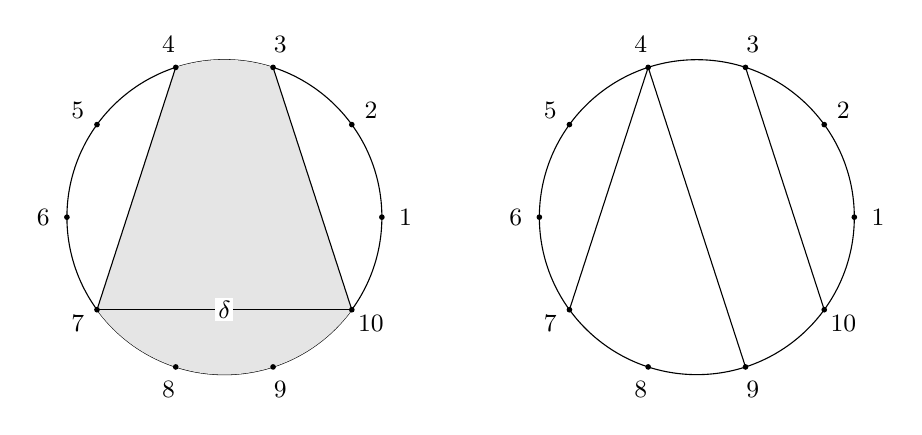
\begin{tikzpicture}[
 scale=2,
 dot/.style={circle,fill=black,inner sep=1.2pt},
 every node/.style={font=\small}
]

% Radius
\def\r{1}

%%%%%%%%%%%%%%%%%%%%%%%%%%%%%%%%%%%%%%%%%%%%%%%%%%%%%%%%%%%%
% Left picture
%%%%%%%%%%%%%%%%%%%%%%%%%%%%%%%%%%%%%%%%%%%%%%%%%%%%%%%%%%%%

\begin{scope}

% Circle
\draw (0,0) circle (\r);

% Coordinates
\foreach \i in {1,...,10}{
 \coordinate (L\i) at ({( \i-1)*36}: \r);
}

% Shaded region
\fill[gray!20]
 (L3)
 arc[start angle=72,end angle=108,radius=\r]
 -- (L7)
 arc[start angle=216,end angle=324,radius=\r]
 -- cycle;

% Chords
\draw (L4)--(L7);
\draw (L7)-- node[midway,fill=white,inner sep=1pt] {$\delta$} (L10);
\draw (L10)--(L3);

% Dots and labels
\foreach \i in {1,...,10}{
 \fill (L\i) circle (0.018);
 \node at ({(\i-1)*36}:1.15) {\i};
}

\end{scope}

%%%%%%%%%%%%%%%%%%%%%%%%%%%%%%%%%%%%%%%%%%%%%%%%%%%%%%%%%%%%
% Right picture
%%%%%%%%%%%%%%%%%%%%%%%%%%%%%%%%%%%%%%%%%%%%%%%%%%%%%%%%%%%%

\begin{scope}[xshift=3cm]

% Circle
\draw (0,0) circle (\r);

% Coordinates
\foreach \i in {1,...,10}{
 \coordinate (R\i) at ({(\i-1)*36}: \r);
}

% Chords
\draw (R4)--(R7);
\draw (R4)--(R9);
\draw (R3)--(R10);

% Dots and labels
\foreach \i in {1,...,10}{
 \fill (R\i) circle (0.018);
 \node at ({(\i-1)*36}:1.15) {\i};
}

\end{scope}
\end{tikzpicture}
\caption{An $n$-angulation $(n=4$, $k=3$, $d_{k,n}=10)$ and its forward flip along the $n$-diagonal $\delta$.}\label{fig:n-diagonal}
\end{figure}


 The cluster exchange graph of $\mathcal{C}_{k,n}$ (with vertices being simple hearts and edges arising from tilts) then has a purely combinatorial description in terms of directed flips of $n$-angulations, cf.~\cite[Theorem~5.6]{Baur-Marsh} or \cite[Theorem~6.3]{Ikeda}.

 The orientation-preserving mapping class group of the marked disc acts (with finite stabilisers) on $n$-angulations and hence on the cluster exchange graph.

 The $A_k$-quiver has an associated ${\rm CY}_n$-category, via the Ginzburg construction, which also has a heart exchange graph. It is a non-trivial theorem of Buan, Reiten and Thomas~\cite{BRT} that one can associate to a heart in the Ginzburg category a `silting collection' in the quotient cluster category, and that this defines a map from the heart exchange graph upstairs to the cluster exchange graph downstairs.
 In \cite[Theorem~8.6]{King-QiuYu-cluster}, the authors show that the braid group acts fibrewise with respect to this map and moreover acts transitively on each fibre. This then establishes all the conditions needed for the argument of \cite[Theorem~9.9]{BS}.
 \end{proof}

\begin{lem}
There is an equivalence $\scrR\bigl(A_k^{(n)}\bigr) \simeq \mathcal{C}_{k,n}$.
\end{lem}

\begin{proof} This is observed \emph{en passant} in the discussion before \cite[Conjecture~1.5]{Lekili-Ueda}. A more detailed identification of the cluster category and Rabinowitz Fukaya category for a Dynkin quiver is given in \cite[Corollary~1.4]{BJK}. \end{proof}

\begin{lem}
 There is a commuting diagram
 \[
\xymatrix{
\Auteq\bigl(\scrF\bigl(A_k^{(n)}\bigr)\bigr) \ar^{\mathrm{Ikeda}}[rr] && \bZ/d_{k,n}\bZ \ar@{=}[d] \\
\Auteq\bigl(\scrW\bigl(A_k^{(n)}\bigr)\bigr) \ar[u] \ar[r] & \Auteq\bigl(\scrR\bigl(A_k^{(n)}\bigr)\bigr) \ar[r] & \bZ/d_{k,n}\bZ.
}
 \]
\end{lem}

\begin{proof}
On any Weinstein manifold, the Rabinowitz Fukaya category is algebraically determined from the wrapped category as the `categorical formal punctured neighbourhood of infinity' (given by quotienting out proper modules), cf.~\cite{GGV} and the definition in Section~\ref{Sec:flavours}, which defines the first arrow on the bottom line. The wrapped and compact Fukaya categories are in this case Koszul dual,\footnote{Since $n\geq 3$, the compact category $\scrF(A_k^{(n)})$ is a Koszul dualising subcategory of $\scrW(A_k^{(n)})$; this follows by combining results of~\cite{AbSm-plumbing} and~\cite{Kalck-Yang}, cf.~the discussion of Koszul duality later in Section~\ref{sec:marked-bordered-surfaces} (which encompasses this case when $n=3$, viewing the $A_k^{(n)}$-Milnor fibres as special cases of the 3-folds associated to marked bordered surfaces; the arguments when $n>3$ are identical).} which defines the left vertical arrow.

Commutativity of the diagram amounts to the fact that both horizontal arrows are given by the action of autoequivalences on the heart exchange graph. In more detail, Ikeda \cite[Section~7]{Ikeda} constructs the top arrow directly using the action on the heart exchange graph. The quotient of the heart exchange graph by the braid group action is identified with the cluster exchange graph of $\scrR\bigl(A_k^{(n)}\bigr)$ by \cite{King-QiuYu-cluster}. Furthermore, the cluster exchange graph is purely combinatorial, as discussed above, and the bottom right map is constructed using the action on the cluster exchange graph.
\end{proof}

\begin{rmk}
 It seems likely that the simplicial automorphism group of the cluster exchange graph is given by the mapping class group of the marked surface, which in this case is just the given cyclic group. This is known in the case of triangulations (here corresponding to the 3-fold case), but does not seem to have been written down for $m$-angulations in general. That would give a more direct argument for the previous result.
\end{rmk}

Since compactly supported symplectomorphisms of $X$ act on both $\scrF$ and $\scrW$ and act trivially on the quotient category $\scrR(X)$, we immediately infer that the composite map
\[
\pi_0\Symp_{\rm ct}(X) \to \Auteq\bigl(\scrF\bigl(A_k^{(n)}\bigr)\bigr) \to \bZ/d_{k,n}\bZ
\]
vanishes, hence the first arrow lifts to ${\rm Br}_{k+1}$, as required.


\begin{thebibliography}{99}
\footnotesize\itemsep=0pt

\bibitem{Abouzaid-Seidel:Viterbo}
Abouzaid M., Seidel P., An open string analogue of {V}iterbo functoriality,
 \href{https://doi.org/10.2140/gt.2010.14.627}{\textit{Geom. Topol.}}
 \textbf{14} (2010), 627--718,
 \href{http://arxiv.org/abs/0712.3177}{arXiv:0712.3177}.

\bibitem{AbSm-plumbing}
Abouzaid M., Smith I., Exact {L}agrangians in plumbings,
 \href{https://doi.org/10.1007/s00039-012-0162-y}{\textit{Geom. Funct. Anal.}}
 \textbf{22} (2012), 785--831,
 \href{http://arxiv.org/abs/1107.0129}{arXiv:1107.0129}.

\bibitem{Akaho-Joyce}
Akaho M., Joyce D., Immersed {L}agrangian {F}loer theory,
 \href{https://doi.org/10.4310/jdg/1303219427}{\textit{J.~Differential Geom.}}
 \textbf{86} (2010), 381--500,
 \href{http://arxiv.org/abs/0803.0717}{arXiv:0803.0717}.

\bibitem{Amiot}
Amiot C., Cluster categories for algebras of global dimension 2 and quivers
 with potential, \href{https://doi.org/10.5802/aif.2499}{\textit{Ann. Inst.
 Fourier (Grenoble)}} \textbf{59} (2009), 2525--2590,
 \href{http://arxiv.org/abs/0805.1035}{arXiv:0805.1035}.

\bibitem{August-Wemyss}
August J., Wemyss M., Stability conditions for contraction algebras,
 \href{https://doi.org/10.1017/fms.2022.65}{\textit{Forum Math. Sigma}}
 \textbf{10} (2022), e73, 20~pages,
 \href{http://arxiv.org/abs/1907.12756}{arXiv:1907.12756}.

\bibitem{Auroux-Smith}
Auroux D., Smith I., Fukaya categories of surfaces, spherical objects and
 mapping class groups,
 \href{https://doi.org/10.1017/fms.2021.21}{\textit{Forum Math. Sigma}}
 \textbf{9} (2021), e26, 50~pages,
 \href{http://arxiv.org/abs/2006.09689}{arXiv:2006.09689}.

\bibitem{BJK}
Bae H., Jeong W., Kim J., Cluster categories from {F}ukaya categories,
 \href{https://doi.org/10.1142/S0129167X25500193}{\textit{Internat.~J. Math.}}
 \textbf{36} (2025), 2550019, 30~pages,
 \href{http://arxiv.org/abs/2209.09442}{arXiv:2209.09442}.

\bibitem{Baur-Marsh}
Baur K., Marsh R.J., A geometric description of {$m$}-cluster categories,
 \href{https://doi.org/10.1090/S0002-9947-08-04441-3}{\textit{Trans. Amer.
 Math. Soc.}} \textbf{360} (2008), 5789--5803,
 \href{http://arxiv.org/abs/math.RA/0607151}{arXiv:math.RA/0607151}.

\bibitem{Birman-Hilden}
Birman J.S., Hilden H.M., On isotopies of homeomorphisms of {R}iemann surfaces,
 \href{https://doi.org/10.2307/1970830}{\textit{Ann. of Math.}} \textbf{97}
 (1973), 424--439.

\bibitem{Blanc}
Blanc J., Symplectic birational transformations of the plane,
 \href{https://doi.org/10.18910/25084}{\textit{Osaka~J. Math.}} \textbf{50}
 (2013), 573--590, \href{http://arxiv.org/abs/1012.0706}{arXiv:1012.0706}.

\bibitem{BEE}
Bourgeois F., Ekholm T., Eliashberg Y., Effect of {L}egendrian surgery (with an
 appendix by {S}heel {G}anatra and {M}aksim {M}aydanskiy),
 \href{https://doi.org/10.2140/gt.2012.16.301}{\textit{Geom. Topol.}}
 \textbf{16} (2012), 301--389,
 \href{http://arxiv.org/abs/0911.0026}{arXiv:0911.0026}.

\bibitem{BS}
Bridgeland T., Smith I., Quadratic differentials as stability conditions,
 \href{https://doi.org/10.1007/s10240-014-0066-5}{\textit{Publ. Math. Inst.
 Hautes \'{E}tudes Sci.}} \textbf{121} (2015), 155--278,
 \href{http://arxiv.org/abs/1302.7030}{arXiv:1302.7030}.

\bibitem{Brustle-YuQiu}
Br\"{u}stle T., Qiu Y., Tagged mapping class groups: {A}uslander--{R}eiten
 translation,
 \href{https://doi.org/10.1007/s00209-015-1405-z}{\textit{Math.~Z.}}
 \textbf{279} (2015), 1103--1120,
 \href{http://arxiv.org/abs/1212.0007}{arXiv:1212.0007}.

\bibitem{Brustle-Zhang}
Br\"{u}stle T., Zhang J., On the cluster category of a marked surface without
 punctures, \href{https://doi.org/10.2140/ant.2011.5.529}{\textit{Algebra
 Number Theory}} \textbf{5} (2011), 529--566,
 \href{http://arxiv.org/abs/1005.2422}{arXiv:1005.2422}.

\bibitem{BRT}
Buan A.B., Reiten I., Thomas H., From {$m$}-clusters to {$m$}-noncrossing
 partitions via exceptional sequences,
 \href{https://doi.org/10.1007/s00209-011-0906-7}{\textit{Math.~Z.}}
 \textbf{271} (2012), 1117--1139,
 \href{http://arxiv.org/abs/1007.0928}{arXiv:1007.0928}.

\bibitem{CPU}
Chan K., Pomerleano D., Ueda K., Lagrangian torus fibrations and homological
 mirror symmetry for the conifold,
 \href{https://doi.org/10.1007/s00220-015-2477-7}{\textit{Comm. Math. Phys.}}
 \textbf{341} (2016), 135--178,
 \href{http://arxiv.org/abs/1305.0968}{arXiv:1305.0968}.

\bibitem{Christ}
Christ M., Ginzburg algebras of triangulated surfaces and perverse schobers,
 \href{https://doi.org/10.1017/fms.2022.1}{\textit{Forum Math. Sigma}}
 \textbf{10} (2022), e8, 72~pages,
 \href{http://arxiv.org/abs/2101.01939}{arXiv:2101.01939}.

\bibitem{DRE}
Dimitroglou~Rizell G., Evans J.D., Exotic spheres and the topology of
 symplectomorphism groups,
 \href{https://doi.org/10.1112/jtopol/jtv007}{\textit{J.~Topol.}} \textbf{8}
 (2015), 586--602, \href{http://arxiv.org/abs/1407.3173}{arXiv:1407.3173}.

\bibitem{Disarlo}
Disarlo V., Combinatorial rigidity of arc complexes,
 \href{http://arxiv.org/abs/1505.08080}{arXiv:1505.08080}.

\bibitem{Dolgachev-book}
Dolgachev I.V., Classical algebraic geometry. {A}~modern view,
 \href{https://doi.org/10.1017/CBO9781139084437}{Cambridge University Press},
 Cambridge, 2012.

\bibitem{Donovan-Wemyss}
Donovan W., Wemyss M., Twists and braids for general 3-fold flops,
 \href{https://doi.org/10.4171/JEMS/868}{\textit{J.~Eur. Math. Soc. (JEMS)}}
 \textbf{21} (2019), 1641--1701,
 \href{http://arxiv.org/abs/1504.05320}{arXiv:1504.05320}.

\bibitem{Drinfeld}
Drinfeld V., D{G} quotients of {DG} categories,
 \href{https://doi.org/10.1016/j.jalgebra.2003.05.001}{\textit{J.~Algebra}}
 \textbf{272} (2004), 643--691,
 \href{http://arxiv.org/abs/math.KT/0210114}{arXiv:math.KT/0210114}.

\bibitem{Evans}
Evans J.D., Symplectic mapping class groups of some {S}tein and rational
 surfaces,
 \href{https://doi.org/10.4310/jsg.2011.v9.n1.a4}{\textit{J.~Symplectic
 Geom.}} \textbf{9} (2011), 45--82,
 \href{http://arxiv.org/abs/0909.5622}{arXiv:0909.5622}.

\bibitem{Fan-Lai}
Fan Y.-W., Lai K.-W., Mirror symmetry for lattice-polarised abelian surfaces,
 \href{http://arxiv.org/abs/2602.04232}{arXiv:2602.04232}.

\bibitem{FST}
Fomin S., Shapiro M., Thurston D., Cluster algebras and triangulated surfaces.
 {I}. {C}luster complexes,
 \href{https://doi.org/10.1007/s11511-008-0030-7}{\textit{Acta Math.}}
 \textbf{201} (2008), 83--146,
 \href{http://arxiv.org/abs/math.RA/0608367}{arXiv:math.RA/0608367}.

\bibitem{GGV}
Ganatra S., Gao Y., Venkatesh S., Rabinowitz {F}ukaya categories and the
 categorical formal punctured neighborhood of infinity,
 \href{http://arxiv.org/abs/2212.14863}{arXiv:2212.14863}.

\bibitem{GPS}
Ganatra S., Pardon J., Shende V., Covariantly functorial wrapped {F}loer theory
 on {L}iouville sectors,
 \href{https://doi.org/10.1007/s10240-019-00112-x}{\textit{Publ. Math. Inst.
 Hautes \'{E}tudes Sci.}} \textbf{131} (2020), 73--200,
 \href{http://arxiv.org/abs/1706.03152}{arXiv:1706.03152}.

\bibitem{Ginzburg}
Ginzbug V., Calabi--{Y}au algebras,
 \href{http://arxiv.org/abs/math.SG/0612139}{arXiv:math.SG/0612139}.

\bibitem{Groman}
Groman Y., Floer theory and reduced cohomology on open manifolds,
 \href{https://doi.org/10.2140/gt.2023.27.1273}{\textit{Geom. Topol.}}
 \textbf{27} (2023), 1273--1390,
 \href{http://arxiv.org/abs/1510.04265}{arXiv:1510.04265}.

\bibitem{Gromov-1985}
Gromov M., Pseudo holomorphic curves in symplectic manifolds,
 \href{https://doi.org/10.1007/BF01388806}{\textit{Invent. Math.}} \textbf{82}
 (1985), 307--347.

\bibitem{GHK2}
Gross M., Hacking P., Keel S., Moduli of surfaces with an anti-canonical cycle,
 \href{https://doi.org/10.1112/S0010437X14007611}{\textit{Compos. Math.}}
 \textbf{151} (2015), 265--291,
 \href{http://arxiv.org/abs/1211.6367}{arXiv:1211.6367}.

\bibitem{Hacking-Keating-1}
Hacking P., Keating A., Homological mirror symmetry for log {C}alabi--{Y}au
 surfaces (with an appendix by {W}endelin {L}utz),
 \href{https://doi.org/10.2140/gt.2022.26.3747}{\textit{Geom. Topol.}}
 \textbf{26} (2022), 3747--3833,
 \href{http://arxiv.org/abs/2005.05010}{arXiv:2005.05010}.

\bibitem{Hacking-Keating-2}
Hacking P., Keating A., Symplectomorphisms of some {W}einstein 4-manifolds,
 \href{https://doi.org/10.2140/gt.2026.30.645}{\textit{Geom. Topol.}}
 \textbf{30} (2026), 645--699,
 \href{http://arxiv.org/abs/2112.06797}{arXiv:2112.06797}.

\bibitem{Hacking-Keating-3}
Hacking P., Keating A., Homological mirror symmetry for projective {K}3,
 \href{http://arxiv.org/abs/2503.05680}{arXiv:2503.05680}.

\bibitem{Hara-Wemyss}
Hara W., Wemyss M., Spherical objects in dimensions two and three,
 \href{https://doi.org/10.4171/jems/1504}{\textit{J.~Eur. Math. Soc. (JEMS)}}
 \textbf{28} (2026), 1771--1808,
 \href{http://arxiv.org/abs/2205.11552}{arXiv:2205.11552}.

\bibitem{Hirano-Wemyss}
Hirano Y., Wemyss M., Stability conditions for 3-fold flops,
 \href{https://doi.org/10.1215/00127094-2022-0097}{\textit{Duke Math.~J.}}
 \textbf{172} (2023), 3105--3173,
 \href{http://arxiv.org/abs/1907.09742}{arXiv:1907.09742}.

\bibitem{Hu-Krah}
Hu X., Krah J., Autoequivalences of blow-ups of minimal surfaces,
 \href{https://doi.org/10.1112/blms.13131}{\textit{Bull. Lond. Math. Soc.}}
 \textbf{56} (2024), 3257--3267,
 \href{http://arxiv.org/abs/2310.17938}{arXiv:2310.17938}.

\bibitem{Ikeda}
Ikeda A., Stability conditions on {${\rm CY}_N$} categories associated to
 {$A_n$}-quivers and period maps,
 \href{https://doi.org/10.1007/s00208-016-1375-4}{\textit{Math. Ann.}}
 \textbf{367} (2017), 1--49,
 \href{http://arxiv.org/abs/1405.5492}{arXiv:1405.5492}.

\bibitem{Ionescu}
Ionescu P., Deformations of complete intersections, \textit{Rev. Roumaine Math.
 Pures Appl.} \textbf{25} (1980), 751--758.

\bibitem{Jacquet-Malo}
Jacquet-Malo L., A bijection between {$m$}-cluster-tilting objects and
 {$(m+2)$}-angulations in {$m$}-cluster categories,
 \href{https://doi.org/10.1016/j.jalgebra.2021.11.041}{\textit{J.~Algebra}}
 \textbf{595} (2022), 581--632,
 \href{http://arxiv.org/abs/1706.06866}{arXiv:1706.06866}.

\bibitem{Jannaud}
Jannaud A., Dehn--{S}eidel twist, ${C}^0$ symplectic topology and barcodes,
 \href{http://arxiv.org/abs/2101.07878}{arXiv:2101.07878}.

\bibitem{Kalck-Yang}
Kalck M., Yang D., Relative singularity categories {I}: {A}uslander
 resolutions, \href{https://doi.org/10.1016/j.aim.2016.06.011}{\textit{Adv.
 Math.}} \textbf{301} (2016), 973--1021,
 \href{http://arxiv.org/abs/1205.1008}{arXiv:1205.1008}.

\bibitem{Karabas-Lee}
Karabas D., Lee S., The wrapped {F}ukaya category of plumbings,
 \href{https://doi.org/10.4310/jsg.250820172316}{\textit{J.~Symplectic Geom.}}
 \textbf{23} (2025), 853--949,
 \href{http://arxiv.org/abs/2405.10783}{arXiv:2405.10783}.

\bibitem{Kartal:algebraic}
Kartal Y.B., Algebraic sheaves of {F}loer homology groups via algebraic torus
 actions on the {F}ukaya category,
 \href{http://arxiv.org/abs/2109.12256}{arXiv:2109.12256}.

\bibitem{Keating-Smith}
Keating A., Smith I., Symplectomorphisms and spherical objects in the conifold
 smoothing, \href{https://doi.org/10.1112/S0010437X24007425}{\textit{Compos.
 Math.}} \textbf{160} (2024), 2738--2773,
 \href{http://arxiv.org/abs/2301.10525}{arXiv:2301.10525}.

\bibitem{KS:corr}
Keating A., Smith I., Corrigendum to ``Symplectomorphisms and spherical objects
 in the conifold smoothing'',
 \href{https://doi.org/10.1017/S0010437X26103297}{\textit{Compos. Math.}}
 \textbf{162} (2026), 1046--1051.

\bibitem{Keating-Ward}
Keating A., Ward A., A universal mirror to $\bigl(\mathbb{P}^2,\Omega\bigr)$ as
 a~birational object,
 \href{http://arxiv.org/abs/2408.03764}{arXiv:2408.03764}.

\bibitem{Keller-Yang}
Keller B., Yang D., Derived equivalences from mutations of quivers with
 potential, \href{https://doi.org/10.1016/j.aim.2010.09.019}{\textit{Adv.
 Math.}} \textbf{226} (2011), 2118--2168,
 \href{http://arxiv.org/abs/0906.0761}{arXiv:0906.0761}.

\bibitem{Khovanov-Seidel}
Khovanov M., Seidel P., Quivers, {F}loer cohomology, and braid group actions,
 \href{https://doi.org/10.1090/S0894-0347-01-00374-5}{\textit{J.~Amer. Math.
 Soc.}} \textbf{15} (2002), 203--271,
 \href{http://arxiv.org/abs/math.QA/0006056}{arXiv:math.QA/0006056}.

\bibitem{King-QiuYu-cluster}
King A., Qiu Y., Exchange graphs and {E}xt quivers,
 \href{https://doi.org/10.1016/j.aim.2015.08.017}{\textit{Adv. Math.}}
 \textbf{285} (2015), 1106--1154,
 \href{http://arxiv.org/abs/1109.2924}{arXiv:1109.2924}.

\bibitem{King-QiuYu}
King A., Qiu Y., Cluster exchange groupoids and framed quadratic differentials,
 \href{https://doi.org/10.1007/s00222-019-00932-y}{\textit{Invent. Math.}}
 \textbf{220} (2020), 479--523,
 \href{http://arxiv.org/abs/1805.00030}{arXiv:1805.00030}.

\bibitem{Lalonde-Pinsonnault}
Lalonde F., Pinsonnault M., The topology of the space of symplectic balls in
 rational 4-manifolds,
 \href{https://doi.org/10.1215/S0012-7094-04-12223-7}{\textit{Duke Math.~J.}}
 \textbf{122} (2004), 347--397,
 \href{http://arxiv.org/abs/math.SG/0207096}{arXiv:math.SG/0207096}.

\bibitem{LS}
Lekili Y., Segal E., Equivariant {F}ukaya categories at singular values,
 \href{https://doi.org/10.1017/s0017089525100487}{\textit{Glasg. Math.~J.}}
 \textbf{68} (2026), 197--221,
 \href{http://arxiv.org/abs/2304.10969}{arXiv:2304.10969}.

\bibitem{Lekili-Ueda}
Lekili Y., Ueda K., Homological mirror symmetry for {M}ilnor fibers via moduli
 of {$A_\infty$}-structures,
 \href{https://doi.org/10.1112/topo.12248}{\textit{J.~Topol.}} \textbf{15}
 (2022), 1058--1106, \href{http://arxiv.org/abs/1806.04345}{arXiv:1806.04345}.

\bibitem{Li-Li-Wu-1}
Li J., Li T.-J., Wu W., The symplectic mapping class group of {$\mathbb
 CP^2\#n\overline{\mathbb CP^2}$} with {$n \le 4$},
 \href{https://doi.org/10.1307/mmj/1434731926}{\textit{Michigan Math.~J.}}
 \textbf{64} (2015), 319--333,
 \href{http://arxiv.org/abs/1310.7329}{arXiv:1310.7329}.

\bibitem{Li-Li-Wu-2}
Li J., Li T.-J., Wu W., Symplectic {$(-2)$}-spheres and the symplectomorphism
 group of small rational 4-manifolds~{II},
 \href{https://doi.org/10.1090/tran/8517}{\textit{Trans. Amer. Math. Soc.}}
 \textbf{375} (2022), 1357--1410,
 \href{http://arxiv.org/abs/1911.11073}{arXiv:1911.11073}.

\bibitem{Li-Li-Wu}
Li J., Li T.-J., Wu W., Symplectic {T}orelli groups of rational surfaces,
 \href{http://arxiv.org/abs/2212.01873}{arXiv:2212.01873}.

\bibitem{Li-Wu}
Li T.-J., Wu W., Lagrangian spheres, symplectic surfaces and the symplectic
 mapping class group,
 \href{https://doi.org/10.2140/gt.2012.16.1121}{\textit{Geom. Topol.}}
 \textbf{16} (2012), 1121--1169,
 \href{http://arxiv.org/abs/1012.4146}{arXiv:1012.4146}.

\bibitem{Looijenga}
Looijenga E., Artin groups and the fundamental groups of some moduli spaces,
 \href{https://doi.org/10.1112/jtopol/jtm009}{\textit{J.~Topol.}} \textbf{1}
 (2008), 187--216,
 \href{http://arxiv.org/abs/math.AG/9801117}{arXiv:math.AG/9801117}.

\bibitem{Lunts-Orlov}
Lunts V.A., Orlov D.O., Uniqueness of enhancement for triangulated categories,
 \href{https://doi.org/10.1090/S0894-0347-10-00664-8}{\textit{J.~Amer. Math.
 Soc.}} \textbf{23} (2010), 853--908,
 \href{http://arxiv.org/abs/0908.4187}{arXiv:0908.4187}.

\bibitem{Margalit-Winarski}
Margalit D., Winarski R.R., Braid groups and mapping class groups: {T}he
 {B}irman--{H}ilden theory,
 \href{https://doi.org/10.1112/blms.12456}{\textit{Bull. Lond. Math. Soc.}}
 \textbf{53} (2021), 643--659.

\bibitem{Munoz-Echaniz}
Mu\~noz Ech\'aniz J., Configurations of {L}agrangian spheres in {$K3$}
 surfaces, \href{http://arxiv.org/abs/2507.15039}{arXiv:2507.15039}.

\bibitem{Okada-Spotti-Sun}
Odaka Y., Spotti C., Sun S., Compact moduli spaces of {D}el {P}ezzo surfaces
 and {K}\"{a}hler--{E}instein metrics,
 \href{https://doi.org/10.4310/jdg/1452002879}{\textit{J.~Differential Geom.}}
 \textbf{102} (2016), 127--172,
 \href{http://arxiv.org/abs/1210.0858}{arXiv:1210.0858}.

\bibitem{Pinsonnault}
Pinsonnault M., Symplectomorphism groups and embeddings of balls into rational
 ruled 4-manifolds,
 \href{https://doi.org/10.1112/S0010437X0700334X}{\textit{Compos. Math.}}
 \textbf{144} (2008), 787--810,
 \href{http://arxiv.org/abs/math.SG/0603310}{arXiv:math.SG/0603310}.

\bibitem{Pomerleano}
Pomerleano D., Intrinsic mirror symmetry and categorical crepant resolutions,
 \href{http://arxiv.org/abs/2103.01200}{arXiv:2103.01200}.

\bibitem{QiuYu:spherical-twist-group}
Qiu Y., Decorated marked surfaces: spherical twists versus braid twists,
 \href{https://doi.org/10.1007/s00208-015-1339-0}{\textit{Math. Ann.}}
 \textbf{365} (2016), 595--633,
 \href{http://arxiv.org/abs/1407.0806}{arXiv:1407.0806}.

\bibitem{Qiu-Woolf}
Qiu Y., Woolf J., Contractible stability spaces and faithful braid group
 actions, \href{https://doi.org/10.2140/gt.2018.22.3701}{\textit{Geom.
 Topol.}} \textbf{22} (2018), 3701--3760,
 \href{http://arxiv.org/abs/1407.5986}{arXiv:1407.5986}.

\bibitem{Reid}
Reid M., The complete intersection of two or more quadrics, {U}niversity of
 Cambridge, 1972, available at
 \url{https://mreid.warwick.ac.uk/3folds/qu.pdf}.

\bibitem{JieRen}
Ren J., Calabi--{Y}au categories and graded quivers with potential,
 \href{http://arxiv.org/abs/2402.03330}{arXiv:2402.03330}.

\bibitem{Ritter}
Ritter A.F., Topological quantum field theory structure on symplectic
 cohomology, \href{https://doi.org/10.1112/jtopol/jts038}{\textit{J.~Topol.}}
 \textbf{6} (2013), 391--489,
 \href{http://arxiv.org/abs/1003.1781}{arXiv:1003.1781}.

\bibitem{Salter}
Salter N., On the monodromy group of the family of smooth quintic plane curves,
 \href{https://doi.org/10.1017/S0017089524000284}{\textit{Glasg. Math.~J.}}
 \textbf{67} (2025), 163--184,
 \href{http://arxiv.org/abs/1610.04920}{arXiv:1610.04920}.

\bibitem{Schmutz}
Schmutz~Schaller P., Mapping class groups of hyperbolic surfaces and
 automorphism groups of graphs,
 \href{https://doi.org/10.1023/A:1002672721132}{\textit{Compositio Math.}}
 \textbf{122} (2000), 243--260.

\bibitem{Seidel_T*S2_unpublished}
Seidel P., Symplectic automorphisms of ${T}^*{S}^2$,
 \href{http://arxiv.org/abs/math.DG/9803084}{arXiv:math.DG/9803084}.


\bibitem{Seidel:graded}
Seidel P., Graded {L}agrangian submanifolds,
 \href{https://doi.org/10.24033/bsmf.2365}{\textit{Bull. Soc. Math. France}}
 \textbf{128} (2000), 103--149.

\bibitem{Seidel:bias}
Seidel P., A~biased view of symplectic cohomology, in Current Developments in
 Mathematics,
 \href{https://doi.org/10.4310/CDM.2006.v2006.n1.a4}{International Press},
 Somerville, MA, 2008, 211--253,
 \href{http://arxiv.org/abs/0704.2055}{arXiv:0704.2055}.

\bibitem{Seidel:FCPLT}
Seidel P., Fukaya categories and {P}icard--{L}efschetz theory, \textit{Zur. Lect. Adv.
 Math.}, \href{https://doi.org/10.4171/063}{European Mathematical Society},
 Z\"urich, 2008.

\bibitem{Seidel_lectures_4Dtwists}
Seidel P., Lectures on four-dimensional {D}ehn twists, in Symplectic
 4-Manifolds and Algebraic Surfaces, \textit{Lecture Notes in Math.}, Vol.~1938, \href{https://doi.org/10.1007/978-3-540-78279-7_4}{Springer}, Berlin,
 2008, 231--267,
 \href{http://arxiv.org/abs/math.SG/0309012}{arXiv:math.SG/0309012}.

\bibitem{Seidel:Flux}
Seidel P., Abstract analogues of flux as symplectic invariants,
 \href{https://doi.org/10.24033/msmf.447}{\textit{M\'em. Soc. Math. Fr.
 (N.S.)}} (2014), 135,
 \href{http://arxiv.org/abs/1108.0394}{arXiv:1108.0394}.

\bibitem{Seidel:categorical_dynamics}
Seidel P., Lectures on categorical dynamics and symplectic topology,
 {U}npublished manuscript, 2014, available at
 \url{http://math.mit.edu/~seidel/}.

\bibitem{Seidel-dilating}
Seidel P., Picard--{L}efschetz theory and dilating {$\mathbb{C}^*$}-actions,
 \href{https://doi.org/10.1112/jtopol/jtv029}{\textit{J.~Topol.}} \textbf{8}
 (2015), 1167--1201, \href{http://arxiv.org/abs/1403.7571}{arXiv:1403.7571}.

\bibitem{Sheridan-Smith:K3}
Sheridan N., Smith I., Symplectic topology of {$K3$} surfaces via mirror
 symmetry, \href{https://doi.org/10.1090/jams/946}{\textit{J.~Amer. Math.
 Soc.}} \textbf{33} (2020), 875--915,
 \href{http://arxiv.org/abs/1709.09439}{arXiv:1709.09439}.

\bibitem{Smith}
Smith I., Floer cohomology and pencils of quadrics,
 \href{https://doi.org/10.1007/s00222-011-0364-1}{\textit{Invent. Math.}}
 \textbf{189} (2012), 149--250,
 \href{http://arxiv.org/abs/1006.1099}{arXiv:1006.1099}.

\bibitem{Smith:quiver}
Smith I., Quiver algebras as {F}ukaya categories,
 \href{https://doi.org/10.2140/gt.2015.19.2557}{\textit{Geom. Topol.}}
 \textbf{19} (2015), 2557--2617,
 \href{http://arxiv.org/abs/1309.0452}{arXiv:1309.0452}.

\bibitem{Smith-Wemyss}
Smith I., Wemyss M., Double bubble plumbings and two-curve flops,
 \href{https://doi.org/10.1007/s00029-023-00828-z}{\textit{Selecta
 Math.~(N.S.)}} \textbf{29} (2023), 29, 62~pages,
 \href{http://arxiv.org/abs/2010.10114}{arXiv:2010.10114}.

\bibitem{Song-Tillmann}
Song Y., Tillmann U., Braids, mapping class groups, and categorical delooping,
 \href{https://doi.org/10.1007/s00208-007-0117-z}{\textit{Math. Ann.}}
 \textbf{339} (2007), 377--393, \href{http://arxiv.org/abs/math.AT/0609597}{arXiv:math.AT/0609597}.

\bibitem{TV}
To\"{e}n B., Vaqui\'e M., Moduli of objects in dg-categories,
 \href{https://doi.org/10.1016/j.ansens.2007.05.001}{\textit{Ann. Sci.
 \'{E}cole Norm. Sup. (4)}} \textbf{40} (2007), 387--444, \href{http://arxiv.org/abs/math.AG/0503269}{arXiv:math.AG/0503269}.

\bibitem{Uehara}
Uehara H., A trichotomy for the autoequivalence groups on smooth projective
 surfaces, \href{https://doi.org/10.1090/tran/7439}{\textit{Trans. Amer. Math.
 Soc.}} \textbf{371} (2019), 3529--3547, \href{http://arxiv.org/abs/1704.00292}{arXiv:1704.00292}.

\bibitem{Wendl}
Wendl C., Strongly fillable contact manifolds and {$J$}-holomorphic foliations,
 \href{https://doi.org/10.1215/00127094-2010-001}{\textit{Duke Math.~J.}}
 \textbf{151} (2010), 337--384, \href{http://arxiv.org/abs/0806.3193}{arXiv:0806.3193}.

\bibitem{Wu}
Wu W., Exact {L}agrangians in {$A_n$}-surface singularities,
 \href{https://doi.org/10.1007/s00208-013-0993-3}{\textit{Math. Ann.}}
 \textbf{359} (2014), 153--168,
 \href{http://arxiv.org/abs/1302.1598}{arXiv:1302.1598}.

\bibitem{Xie-Li}
Xie B., Li Y., Plumbings of {L}ens spaces and crepant resolutions of compound
 {${A}_n$}-singularities,
 \href{http://arxiv.org/abs/2511.22837}{arXiv:2511.22837}.

\end{thebibliography}
\end{document}
